\documentclass{article}
%%%%%%%%%%%%%%%%%%%%%%%%%%%%%%%%%%%%%%%%%%%%%%%%%%%%%%%%%%%%%%%%%%%%%%%%%%%%%%%%%%%%%%%%%%%%%%%%%%%%%%%%%%%%%%%%%%%%%%%%%%%%%%%%%%%%%%%%%%%%%%%%%%%%%%%%%%%%%%%%%%%%%%%%%%%%%%%%%%%%%%%%%%%%%%%%%%%%%%%%%%%%%%%%%%%%%%%%%%%%%%%%%%%%%%%%%%%%%%%%%%%%%%%%%%%%
\usepackage{eurosym}
\usepackage[top=1cm,bottom=2cm,left=1.5cm,right=1.5cm,a4paper]{geometry}
\usepackage{amsmath,amssymb,mathrsfs}
\usepackage{amsthm}
\usepackage[colorlinks]{hyperref}
%\usepackage[nameinlink]{cleveref}
\usepackage{url}
\usepackage{graphicx,color,epsfig}
\usepackage{epstopdf}
\usepackage{amsfonts}
\usepackage{caption}
\usepackage{enumerate}
\usepackage{enumitem}
\usepackage{float}
\usepackage{booktabs}
\usepackage{graphicx}
\usepackage{caption}
\usepackage{subcaption}
\usepackage{array}
\usepackage{booktabs}
\usepackage{fancyhdr}
\usepackage{eurosym}
\usepackage{cite}
\usepackage{cleveref}
\usepackage{upgreek}
\usepackage{enumitem}
\usepackage{xcolor,rotating}
\usepackage{placeins}
\usepackage{color,soul}
\setcounter{MaxMatrixCols}{10}
%TCIDATA{OutputFilter=Latex.dll}
%TCIDATA{Version=5.50.0.2953}
%TCIDATA{<META NAME="SaveForMode" CONTENT="1">}
%TCIDATA{BibliographyScheme=Manual}
%TCIDATA{LastRevised=Thursday, April 25, 2019 13:23:17}
%TCIDATA{<META NAME="GraphicsSave" CONTENT="32">}
%\renewcommand{\tablename}{{\small F}\scriptsize{IGURE}}
\DeclareMathOperator{\sech}{sech}
\DeclareMathOperator{\csch}{csch}
\newtheorem{theorem}{Theorem}
\newtheorem{acknowledgement}[theorem]{Acknowledgement}
\newtheorem{conclusion}[theorem]{Conclusion}
\newtheorem{condition}[theorem]{Condition}
\newtheorem{corollary}[theorem]{Corollary}
\newtheorem{definition}[theorem]{Definition}
\newtheorem{lemma}[theorem]{Lemma}
\newtheorem{proposition}[theorem]{Proposition}
\newtheorem{remark}[theorem]{Remark}
%\newenvironment{proof}[1][Proof]{\noindent\textbf{#1.} }{\ \rule{0.5em}{0.5em}}
\usepackage[symbol]{footmisc}
\def\correspondingauthor{\footnote{Corresponding author.}}
\numberwithin{equation}{section}
\newlist{steps}{enumerate}{1}
\setlist[steps, 1]{label = Step \arabic*:}
\usepackage{multicol}
\hypersetup{pdftitle={},% title
    pdfauthor={Lanre Akinyemi},     % author
    %pdfsubject={Differential Equations},   % subject of the document
    pdfcreator={pdftex},   % creator of the document
    pdfproducer={Texmaker}, % producer of the document
    pdfkeywords={}, % list of keywords
    colorlinks=true,       % false: boxed links; true: colored links
    linkcolor=blue,          % color of internal links
    citecolor=blue,        % color of links to bibliography
    filecolor=magenta,      % color of file links
    urlcolor=blue           % color of external links
}
\setcounter{MaxMatrixCols}{10}
%%%%%%%%%%%%%%%%%%%%%%%%%%%%%%%%%%%%
\newcommand{\capu}{\mathcal{D}}
%%%%%%%%%%%%%%%%%%%%%%%%%%%%%%%%%%%%
\renewcommand{\equationautorefname}{Eq.}
\Crefname{figure}{Fig.}{Figs.}
\Crefname{table}{Tab.}{Tabs.}
\makeatletter
\let\oldtheequation\theequation
\renewcommand\tagform@[1]{\maketag@@@{\ignorespaces#1\unskip\@@italiccorr}}
\renewcommand\theequation{(\oldtheequation)}
\makeatother
%%%%%%%%%%%%%%%%%%%%%%%%%%%%%%%%%%%
%\newtheorem{theorem}{Theorem}[section]
\newtheorem{case}{Case}
%\newtheorem{definition}[theorem]{Definition}
%\newtheorem{example}[theorem]{Example}
%\newtheorem{lemma}[theorem]{Lemma}
%\newtheorem{remark}[theorem]{Remark}
%\newenvironment{proof}[1][Proof]{\noindent\textbf{#1.} }{\ \rule{0.5em}{0.5em}}
\usepackage[symbol]{footmisc}
\renewcommand{\baselinestretch}{1.2}
%%%%%%%%%%%%%%%%%%%%%%%%%%%%%%%%%%%%
\date{}
%opening\def\correspondingauthor{\footnote{Corresponding author.}}
\begin{document}
\title{ \textbf{Analytical soliton solutions of the non-linear schr\"{o}dinger equation via a simple auxiliary method along with bifurcation analysis } }
\author{ Ali Akg\"{u}l$^{1,2,*}$, Farrah Ashraf $^{3}$, Rehan Khursheed $^{4}$, Romana Ashraf $^{3}$ \\
$^{1}$ Department of Electronics and Communication Engineering,\\ Saveetha School of Engineering,
SIMATS, Chennai, Tamilnadu, India.\\
$^{2}$ Siirt University, Art and Science Faculty, Department of Mathematics, 56100 Siirt, Türkiye.\\
$^{3}$ Department of Computer Science $ \& $ IT,\\ The University of Lahore, Lahore, Pakistan.\\
$^{4}$ Department of Mathematics and Statistics,\\ The University of Lahore, Lahore, Pakistan.\\
Corresponding (*): aliakgul00727@gmail.com\\
e-mail: \{f.as70000, rehankhursheed468, dr.romanauetian\}@gmail.com }
\date{ }
\maketitle
% !TeX spellcheck = en_US
\begin{abstract}
\noindent
 The (NLSE) Non-Linear Schr\"{o}dinger Equation plays a critical role in describing various non-linear wave phenomena in fields such as non-linear optics, plasma physics and fluid dynamics. This article explores the analytical soliton solutions of the NLSE using the (SAM) Simple Auxiliary Method which is a systematic and efficient approach for solving non-linear partial differential equations. The SAM simplifies the complex non-linear structure of the NLSE by introducing an auxiliary function which leads one to the derivation of exact soliton solutions. This method effectively produces bell-shaped solitons, singular solitons, dark solitons, bright solitons, and some periodic solitons for non-linear Schr\"{o}dinger equation. The method’s simplicity and general applicability make it a valuable tool for obtaining explicit solutions of the NLSE providing deeper insights into the dynamics of non-linear waves. This study highlights the power of the Simple Auxiliary Method in analyzing and understanding soliton behaviors with its implications for real-world applications in non-linear wave systems. Appropriate values are given to the parameters involved in the solutions of the equation for graphical view of our results. Our results demonstrate the effectiveness, efficiency and desirability of this differential equation method (SAM) in obtaining good results in solving many different differential equations. The bifurcation analysis of the auxiliary NLSE was carried out through its traveling--wave reduction, which transforms the PDE
into a planar Hamiltonian system. Equilibria and their stability depend on the parameters $A = p^2 + r$ and $B = 2\gamma$, and qualitative changes occur when their signs vary. For $A>0, B>0$, both solitary pulse (homoclinic) and periodic wave solutions coexist. When $A>0, B<0$, only separatrix--type connections remain, eliminating periodic structures. In contrast, $A<0, B<0$ gives rise to kink/antikink (heteroclinic) fronts along with periodic traveling waves, while $A<0, B>0$ supports exclusively periodic waves. These bifurcation regimes provide a complete classification of coherent structures admitted by the NLSE, linking parameter signs to the existence of solitary, periodic and front-type solutions.
\end{abstract}
\textbf{Key words}: Auxiliary equation method, Schr\"{o}dinger equation, Bifurcation, Phase portrait, Analytical soliton solution, Dark soliton, Bright soliton, Singular soliton and Kink shaped solitons.
\section{Introduction}
\noindent The study of solitons and their properties has become a cornerstone of modern mathematical physics particularly in the context of non-linear partial differential equations (PDEs). Among these, the Non-Linear Schr\"{o}dinger Equation (NLSE) stands out as one of the most important equations widely studied in the context of fluid dynamics, non-linear optics and plasma physics. Solitons as stable wave-like solutions of non-linear equations offer unique insights into the behavior of complex systems where wave propagation is governed by both dispersive and non-linear effects. Solitons are non-linear waves. A soliton is considered as solitory traveling wave pulse solution of non-linear partial differential equations. There is non-linear wave phenomena in several areas including blood physics.\cite{A1,A2,A3}, optical fiber \cite{a4,a5,a6,a7}, fluid dynamics \cite{a8,a9} and other non-linear wave phenomena we can get by finding the exact solutions of the non-linear partial differential equations. In the study of non-linear phenomena the solution to these non-linear partial differential equations is crucial. Numerous techniques have been developed in recent years to solve NPDE's such as the $G/G^{'}$ - Expansion method \cite{a8}, Backscatter method \cite{a10}, The Exponential Function method \cite{a11}, Homotopy perturbation method \cite{a12}, Hirota bilinear method \cite{a13}, Homogeneous balance method \cite{a14}, Backlund transform \cite{a15}, and Jacobi and Weierstrass elliptic function method \cite{a16} etc.\\\
The Simple Auxiliary Method is a relatively new and elegant approach that allows for the construction of exact solutions to non-linear equations by introducing an auxiliary function which simplifies the problem without losing the essential non-linear character. This method has gained attention due to its simplicity, general applicability and ability to produce a wide range of soliton solutions including solitary waves, dark and bright waves and kink solutions. By transforming the original non-linear equation into a simpler form using an auxiliary function. This method makes it possible to derive explicit analytical solutions for complex non-linear problems that offers a deeper understanding of the dynamics described by the non-linear Schr\"{o}dinger equation.\\\
The non-linear Schr\"{o}dinger equation has this form \cite{a17}:
\begin{eqnarray}
i u_{t}+u_{\mathit{xx}}\pm 2 \gamma  {| u |}^{2} u = 0,
\end{eqnarray}
Where $\gamma\neq {0}$ and is a real constant and a complex-valued function of two real variable x and t is u = u (x,t). The Schr\"{o}dinger equation is used in many areas of physics including superconductivity, non-linear optics, quantum mechanics and plasma physics \cite{a18}. Isolated solutions are indicated by the NLSE (1.1). These are referred to as NLS ''+'' and NLS ''-'' equivalent circumstances. Non-linear Schr\"{o}dinger positive and Non-linear Schr\"{o}dinger negative have different overlaps. The NLS ''+'' and NLS ''-'' overlaps are not the same. For instance, NLS ''-'' has a dark resolution while NLS ''+'' has a bright one resolution \cite{a19}. Such behavior occurs when there is no conflict between the two plasma instabilities \cite{a20} and the two layers of baroclinic instability \cite{a21}.\\
The unstable non-linear Schr\"{o}dinger (UNLS) equation takes the form:
\begin{eqnarray}
\mathit{iu}_{t}+u_{\mathit{xx}}+2 \gamma  {| u |}^{2} u -2 \gamma  u =  0.
\end{eqnarray}
Vadati et al.\cite{a22} A similar Hamiltonian complex has been proposed as a modification of the amplitude equation (UNLS).
\begin{eqnarray}
\mathit{iu}_{t}+u_{\mathit{xx}}+2 \gamma  {| u |}^{2} u -\epsilon  u_{\mathit{xt}} =  0.
\end{eqnarray}
Identifies some instabilities of the modulated wave train \cite{a23}.\\\
The time-dependent two-dimensional NLSE :
\begin{eqnarray}
\mathit{iu}_{t}+u_{\mathit{xx}}+u_{\mathit{yy}}+\gamma  {| u |}^{2} u =  0.
\end{eqnarray}
This type of equation, which simulates an electromagnetic wave equation in a two-dimensional weakly guiding structure, is found in many areas of physics, including quantum mechanics \cite{a24}, Electromagnetic Wave Propagation \cite{a25}, Underwater Acoustics \cite{a26} and  and the design of specific optoelectronic devices \cite{a27} Because it simulates the electromagnetic wave balance in a two-dimensional weak conductor model. It is also used in many quantum dynamics calculations \cite{a28}.\\\
The time-dependent 3D NLSE non-linear Schr\"{o}dinger equation is expressed as:
\begin{eqnarray}
i u_{t}+u_{\mathit{xx}}+u_{\mathit{yy}}+u_{\mathit{zz}}+\gamma  {| u |}^{2} u =  0.
\end{eqnarray}
Gagnon and Winternitz reported symmetry reductions of the (3 + 1)-dimensional non-linear Schr\"{o}dinger equation in a number of publications \cite{a29,a30,a31,a32,a33}.\\
\section{The Simple Auxiliary Method }
\subsection{Steps of the Simple Auxiliary Method}
The followings are the steps involved in the SAM:\\\
\textbf{\textbf{$1^{st}$} Step:}\\
We use the transformation equation
to convert the (NLPDE) non-linear partial differential equation
\begin{eqnarray}\label{NLPDE}
H(u,u_x,u_y,u_t,u_{xy},........)=0,
\end{eqnarray}
into (ODE) ordinary differential equation form (By uniting the independent variables we get).
\begin{eqnarray}\label{ODE}
G(U,U',U'',U''',.............)=0.
\end{eqnarray}\\\
\textbf{\textbf{$2^{nd}$} Step:}\\
 We now examine the solution to the equation of the following form:
\begin{eqnarray}\label{TF}
U \! \left(\zeta \right)= a_{0} + a_{1} Q \! \left(\zeta \right)+ a_{2} {U \! \left(\zeta \right)}^{2} +........+a_{N} {Q \! \left(\zeta \right)}^{N}.
\end{eqnarray}
\textbf{\textbf{$3^{rd}$} Step:}\\
To obtain the value of N we now use the principles of homogeneous equilibrium and balance which takes into account the highest order derivative term and non-linear factor involved in Eq. \ref{ODE}.
\begin{eqnarray}\label{DV}
\frac{d}{d \zeta}Q \! \left(\zeta \right) =\sqrt{a Q \! \left(\xi \right)^{2}+b Q \! \left(\xi \right)^{3}+c Q \! \left(\xi \right)^{4}},
\end{eqnarray}
where a,b,and c are parameter (real valued).\\\\
\textbf{\textbf{$4^{th}$} Step:}\\
Substitute Eq. \ref{DV} and using the transformation in Eq. \ref{ODE} we get a resulting algebraic equation in ${Q(\zeta)}$. Now we simplify our resulting equation to get the coefficients of all powers of ${Q(\zeta)}$ and then put all the coefficients of all powers of $Q{(\zeta)}$ equal to zero. This will create a system of equations that can be solved separately and simultaneously.\\\
The exact solutions of Eq. \ref{DV} using ${\epsilon=\pm1}$ are:\\\\
\textbf{Family I: for $a > 0$ }
\begin{eqnarray}\label{F1}
Q \! \left(\zeta \right) = -\frac{a b\,\mathrm{sech}\! \left(\frac{\sqrt{a}\, \xi}{2}\right)^{2}}{b^{2}-a c \left[1+\epsilon  \tanh \! \left(\frac{\sqrt{a}\, \xi}{2}\right)\right]^{2}}.
\end{eqnarray}
\textbf{Family II: for $a > 0$ }
\begin{eqnarray}\label{F2}
Q \! \left(\zeta \right) = \frac{a b\,\mathrm{csch}\! \left(\frac{\sqrt{a}\, \xi}{2}\right)^{2}}{b^{2}-a c \left[1+\epsilon  \coth \! \left(\frac{\sqrt{a}\, \xi}{2}\right)\right]^{2}}.
\end{eqnarray}
\textbf{Family III: for $a > 0$ , \,$b^{2}-4ac > 0$ }
\begin{eqnarray}\label{F3}
Q \! \left(\zeta \right) =\frac{2 a \,\mathrm{sech}\! \left(\sqrt{a}\, \xi \right)}{\epsilon  \sqrt{-4 a c +b^{2}}-b \,\mathrm{sech}\! \left(\sqrt{a}\, \xi \right)}.
\end{eqnarray}
\textbf{Family IV: for $a < 0$ , \,$b^{2}-4ac > 0$ }
\begin{eqnarray}\label{F4}
Q \! \left(\zeta \right) =\frac{2 a \sec \! \left(\sqrt{-a}\, \xi \right)}{\epsilon  \sqrt{-4 a c +b^{2}}-b \sec \! \left(\sqrt{-a}\, \xi \right)}.
\end{eqnarray}
\textbf{Family V: for $a > 0$ , \,$b^{2}-4ac < 0$ }
\begin{eqnarray}\label{F5}
Q \! \left(\zeta \right) =\frac{2 a \,\mathrm{csch}\! \left(\sqrt{a}\, \xi \right)}{\epsilon  \sqrt{4 a c -b^{2}}-b \,\mathrm{csch}\! \left(\sqrt{a}\, \xi \right)}.
\end{eqnarray}
\textbf{Family VI: for $a < 0$ , \,$b^{2}-4ac > 0$ }
\begin{eqnarray}\label{F6}
Q \! \left(\zeta \right) =\frac{2 a \csc \! \left(\sqrt{-a}\, \xi \right)}{\epsilon  \sqrt{-4 a c +b^{2}}-b \csc \! \left(\sqrt{-a}\, \xi \right)}.
\end{eqnarray}
\textbf{Family VII: for $a > 0$ , \,$c > 0$ }
\begin{eqnarray}\label{F7}
Q \! \left(\zeta \right) =-\frac{a \mathrm{sech}\! \left(\frac{\sqrt{a}\, \xi}{2}\right)^{2}}{b +2\,\epsilon  \sqrt{a c}\, \tanh \! \left(\frac{\sqrt{a}\, \xi}{2}\right)}.
\end{eqnarray}
\textbf{Family VIII: for $a < 0$ , \,$c > 0$ }
\begin{eqnarray}\label{F8}
Q \! \left(\zeta \right) =-\frac{a \left[\sec^{2}\left(\frac{\sqrt{-a}\, \xi}{2}\right)\right]}{b +2\,\epsilon  \sqrt{-a c}\, \tan \! \left(\frac{\sqrt{-a}\, \xi}{2}\right)}.
\end{eqnarray}
\textbf{Family IX: for $a > 0$ , \,$c > 0$   }
\begin{eqnarray}\label{F9}
Q \! \left(\zeta \right) =\frac{a \mathrm{csch}\! \left(\frac{\sqrt{a}\, \xi}{2}\right)^{2}}{b +2\,\epsilon  \sqrt{a c}\, \coth \! \left(\frac{\sqrt{a}\, \xi}{2}\right)}.
\end{eqnarray}
\textbf{Family X: for $a < 0$ , \,$c > 0$ }
\begin{eqnarray}\label{F10}
Q \! \left(\zeta \right) =-\frac{a \left[\csc^{2}\left(\frac{\sqrt{-a}\, \xi}{2}\right)\right]}{b +2\,\epsilon  \sqrt{-a c}\, \cot \! \left(\frac{\sqrt{-a}\, \xi}{2}\right)}.
\end{eqnarray}
\textbf{Family XI: for $a > 0$ , \,$b^{2}-4ac = 0$  }
\begin{eqnarray}\label{F11}
Q \! \left(\zeta \right) =-\frac{a \left[1+\epsilon  \tanh \! \left(\frac{\sqrt{a}\, \xi}{2}\right)\right]}{b}.
\end{eqnarray}
\textbf{Family XII: for  $a > 0$ , \,$b^{2}-4ac = 0$ }
\begin{eqnarray}\label{F12}
Q \! \left(\zeta \right) =-\frac{a \left[1+\epsilon  \coth \! \left(\frac{\sqrt{a}\, \xi}{2}\right)\right]}{b}.
\end{eqnarray}
\textbf{Family XIII: for $a > 0$ }
\begin{eqnarray}\label{F13}
Q \! \left(\zeta \right) =\frac{4 a \,{\mathrm e}^{\epsilon  \sqrt{a}\, \zeta}}{\left({\mathrm e}^{\epsilon  \sqrt{a}\, \zeta}-b \right)^{2}-4 a c}.
\end{eqnarray}
\textbf{Family XIV:  for $a > 0$ ,\, $b = 0$  }
\begin{eqnarray}\label{F14}
Q \! \left(\zeta \right) =\frac{\left(\pm 4\right) a \epsilon  \,{\mathrm e}^{\epsilon  \sqrt{a}\, \zeta}}{1-4 a c \,{\mathrm e}^{4 \epsilon  \sqrt{a}\, \zeta}}.
\end{eqnarray}
\section{Solution of Non-Linear Schr\"{o}dinger Equation }
Consider NLSE with this form:
\begin{eqnarray}\label{NLSE}
i u_{t}+u_{\mathit{xx}}+2 \gamma  {| u |}^{2} u = 0,
\end{eqnarray}
Now we use this transformation equation
 \begin{eqnarray}\label{TFN}
u \! \left(x , t\right) ={\mathrm e}^{i\theta} U \! \left(\zeta \right),   \qquad \zeta = x + v t,  \qquad \theta = p x + r t.
\end{eqnarray}
and using the relation $v=-2p$ we get
\begin{eqnarray}\label{ODE1}
U^{''}{(\zeta)}-\left(p^{2}+r \right) U \! \left(\zeta \right)+2 \gamma \! \left(U \! \left(\zeta \right)\right)^{3}=0.
\end{eqnarray}
the ODE form of the Schr\"{o}dinger equation. N= 1 is now obtained by balancing the highest degree non-linear term $U^{3}$ and the maximum order derivative term $U''$.\\\
Using $N=1$ in Eq. \ref{TF} will gives:
\begin{eqnarray}\label{S}
U \! \left(\zeta \right)= a_{0} + a_{1} Q \! \left(\zeta \right),
\end{eqnarray}
Here we need to find the constants involved in $U{(\zeta)}$ which are $a_{0}$ and $a_{1}$.\\\
The $Q{(\zeta)}$ represents (the families given) the solutions Eq. \ref{DV}. Now by putting Eq. \ref{TFN}, \ref{S} in Eq. \ref{ODE1} After this we simplify our resulting equation to get the coefficients of all powers of ${Q(\zeta)}$ and then put all the coefficients of all non zero powers of $Q{(\zeta)}$ equal to zero. This will create a set of algebraic equations. These equations can be solved separately or simultaneously.\\\
The non-linear algebraic equations are:\\\
\begin{align}
\begin{cases}
Q^{3}{(\zeta)}:\qquad2 \gamma  a_{1}^{3}+2 a_{1} c = 0,\\\
Q^{2}{(\zeta)}:\qquad\frac{3}{2} a_{1} b +6 \gamma  a_{0} a_{1}^{2} = 0,\\\
Q^{1}{(\zeta)}:\qquad6 \gamma  a_{0}^{2} a_{1}-a_{1} p^{2}+a_{1} a -a_{1} r = 0,\\\
Q^{0}{(\zeta)}:\qquad2 \gamma  a_{0}^{3}-a_{0} p^{2}-a_{0} r = 0.\\\
\end{cases}
\end{align}
By using Maple software we obtained the solution of these equations.\\\
\textbf{Set:}\\\
$a_{0} = -\frac{b}{4 \sqrt{-\gamma  c}}$, \,$a_{1} = \frac{\sqrt{-\gamma  c}}{\gamma}$ and  \,$\nu = - 5\times 10^{-1} \sqrt{-\frac{6 b^{2}}{c}+16 a -16 r}$.\\\
\textbf{ Solution of Set:}\\\
Using Eq. \ref{TFN}, \ref{F1}, \ref{F2}, \ref{F11} and \ref{F12} in Eq. \ref{S} we get the following results:
\begin{eqnarray}\label{U1}
U_{1}\left(\zeta \right) =-\frac{b}{4 \sqrt{-\gamma  c}}-\frac{\sqrt{c (-\gamma)}\, a b\, \mathrm{sech} \left[\frac{\sqrt{a}\, \left(t v +x \right)}{2}\right]^{2}}{\gamma  \left[b^{2}-a c \left(1+\epsilon  \tanh  \left(\frac{\sqrt{a}\, \left(t v +x \right)}{2}\right)\right)^{2}\right]}.
\end{eqnarray}
\begin{eqnarray}\label{U2}
U_{2}\left(\zeta \right) =-\frac{b}{4 \sqrt{-\gamma  c}}+\frac{\sqrt{-\gamma  c}\, a b\, \mathrm{csch} \left[\frac{\sqrt{a}\, \left(t v +x \right)}{2}\right]^{2}}{\gamma  \left[b^{2}-a c \left(1+\epsilon  \coth  \left(\frac{\sqrt{a}\, \left(t v +x \right)}{2}\right)\right)^{2}\right]}.
\end{eqnarray}
\begin{eqnarray}\label{U3}
U_{3}\left(\zeta \right) =-\frac{b}{4 \sqrt{-\gamma  c}}-\frac{\sqrt{-\gamma  c}\, a \left[1+\epsilon  \tanh  \left(\frac{\sqrt{a}\, \left(t v +x \right)}{2}\right)\right]}{\gamma  b}.
\end{eqnarray}
\begin{eqnarray}\label{U4}
U_{4}\left(\zeta \right) =
-\frac{b}{4 \sqrt{-\gamma  c}}-\frac{\sqrt{-\gamma  c}\, a \left[1+\epsilon  \coth \left(\frac{\sqrt{a}\, \left(t v +x \right)}{2}\right)\right]}{\gamma  b}.
\end{eqnarray}
\newpage
\section{The Graphical Representation}
\textbf{Set:}\\\
Using $a = 2$, $b = 3$, $c = -4$, $r = 1.5$ and $\epsilon =1$ the graphical representation of the solutions $U_{1}$, $U_{2}$, $U_{3}$ and $U_{4}$ are
\begin{figure}[h!]
    \centering
    \begin{tabular}{ccc}
        \begin{minipage}{.30\textwidth} 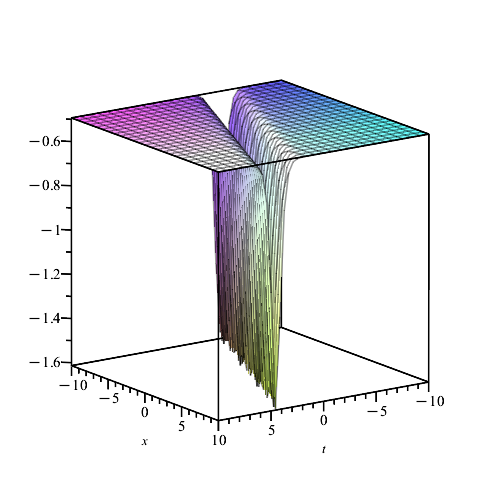
\includegraphics[width=\linewidth,
        height=55mm]{u1.png}\subcaption{} \end{minipage} & \begin{minipage}{.30\textwidth}
            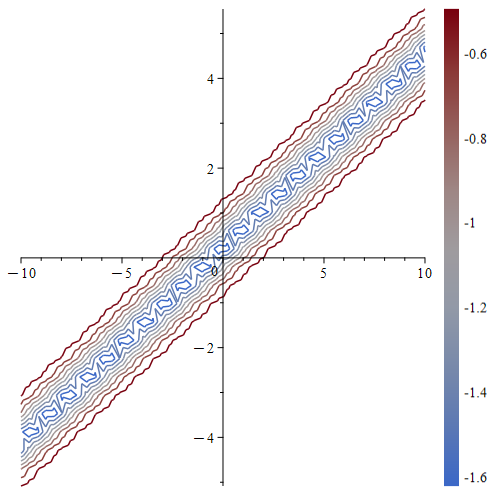
\includegraphics[width=\linewidth, height=55mm]{c1.png}\subcaption{} \end{minipage} & \begin{minipage}{.30\textwidth}
           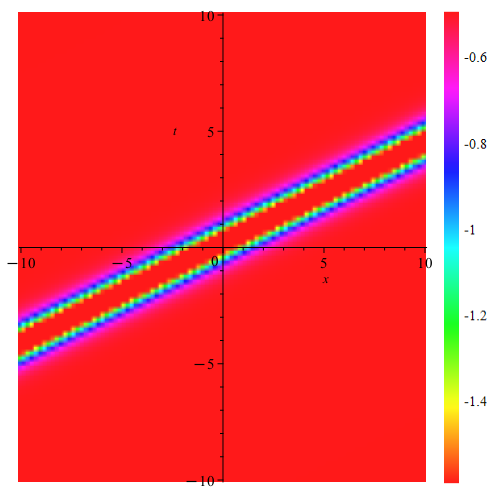
\includegraphics[width=\linewidth, height=55mm]{d1.png}\subcaption{} \end{minipage}
    \end{tabular}%
\caption{The 3D, 2D and Density plot of $U_1(\xi)$ given by Eq. \ref{U1} are shown}.\label{P1}
\end{figure}
\begin{figure}[h!]
    \centering
    \begin{tabular}{ccc}
        \begin{minipage}{.30\textwidth} 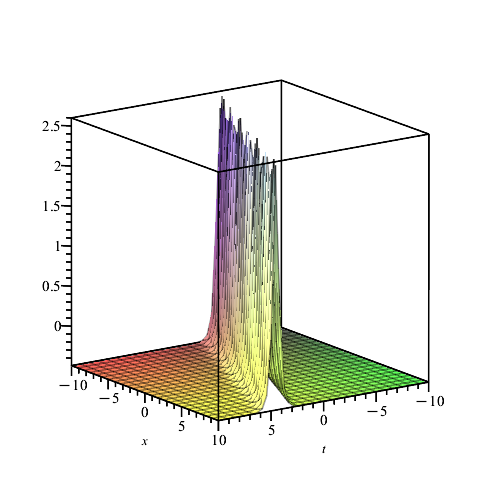
\includegraphics[width=\linewidth,
            height=55mm]{u2.png}\subcaption{} \end{minipage} $\&$ \begin{minipage}{.30\textwidth}
            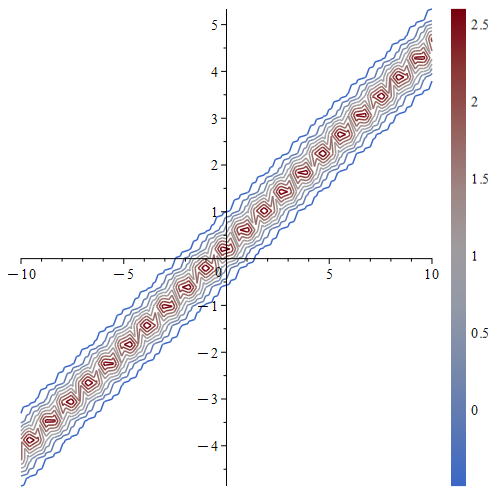
\includegraphics[width=\linewidth, height=55mm]{c2.png}\subcaption{} \end{minipage} & \begin{minipage}{.30\textwidth}
            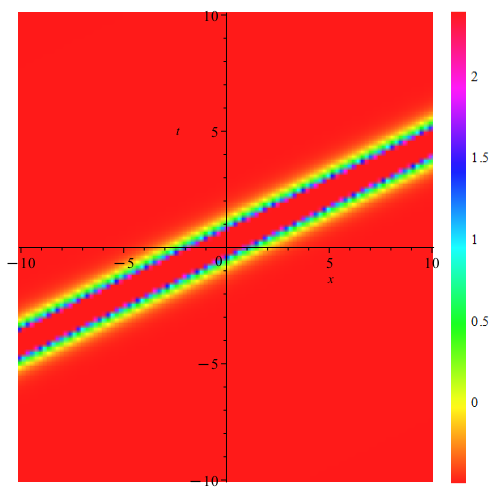
\includegraphics[width=\linewidth, height=55mm]{d2.png}\subcaption{} \end{minipage}
    \end{tabular}%
 \noindent\caption{The 3D, 2D and Density plots of $U_2(\xi)$ given by Eq. \ref{U2}.}\label{P2}
\end{figure}
\begin{figure}[h!]
    \centering
    \begin{tabular}{ccc}
        \begin{minipage}{.30\textwidth} 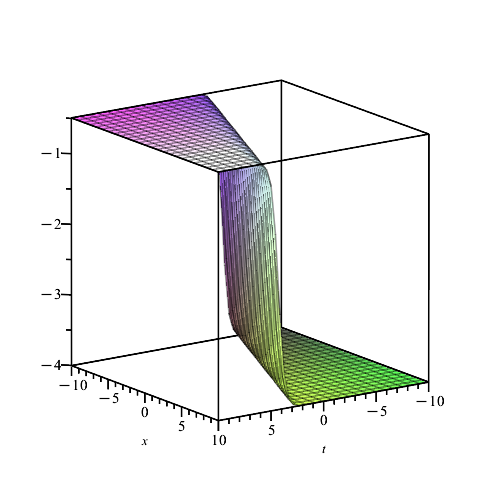
\includegraphics[width=\linewidth,
            height=55mm]{u3.png}\subcaption{} \end{minipage} & \begin{minipage}{.30\textwidth}
            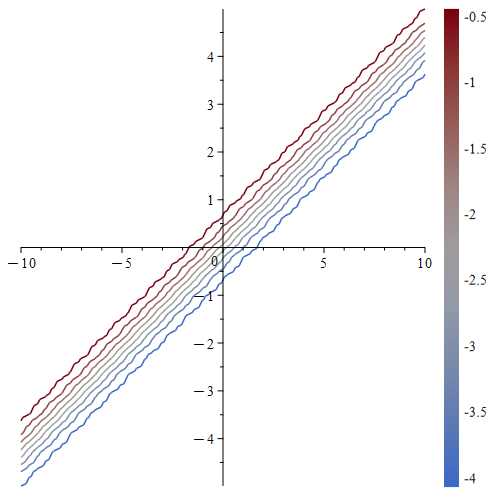
\includegraphics[width=\linewidth, height=55mm]{c3.png}\subcaption{} \end{minipage} & \begin{minipage}{.30\textwidth}
            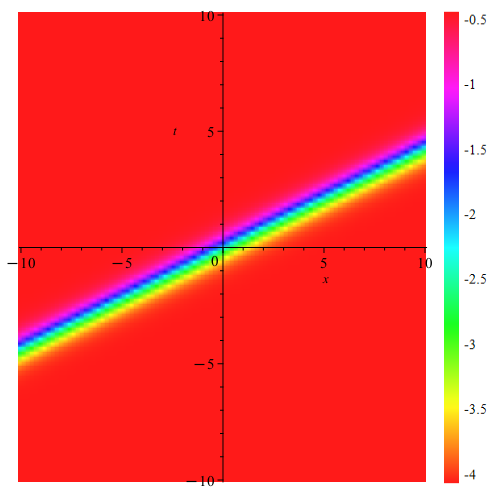
\includegraphics[width=\linewidth, height=55mm]{d3.png}\subcaption{} \end{minipage}
    \end{tabular}%
 \noindent\caption{The 3D, 2D Contour and Density plots of $U_3(\xi)$ given by Eq. \ref{U3}.}\label{P3}
\end{figure}
\begin{figure}[h!]
    \centering
    \begin{tabular}{ccc}
        \begin{minipage}{.30\textwidth} 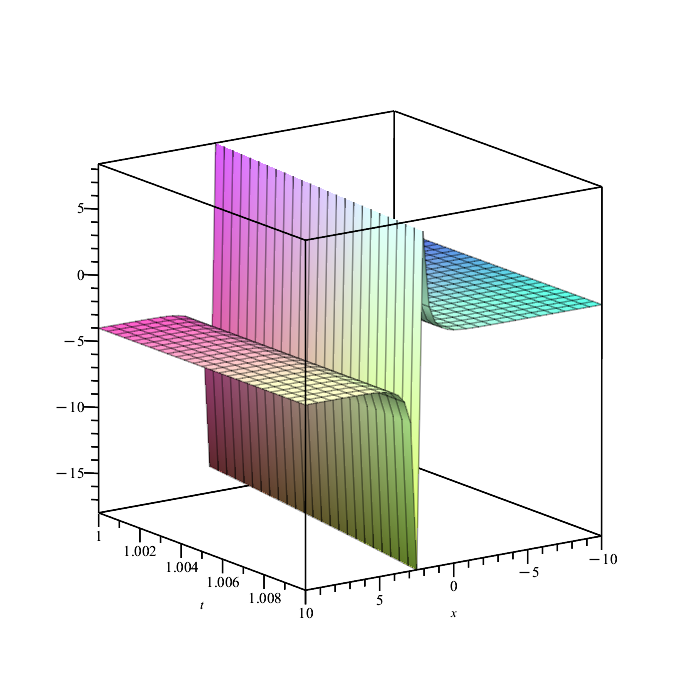
\includegraphics[width=\linewidth,
            height=55mm]{u4.png}\subcaption{} \end{minipage} & \begin{minipage}{.30\textwidth}
            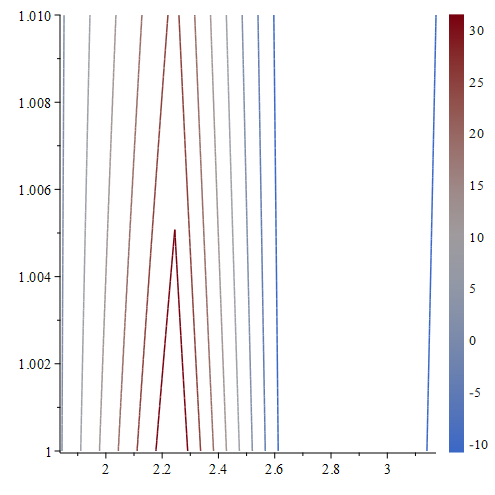
\includegraphics[width=\linewidth, height=55mm]{c4.png}\subcaption{} \end{minipage} & \begin{minipage}{.30\textwidth}
            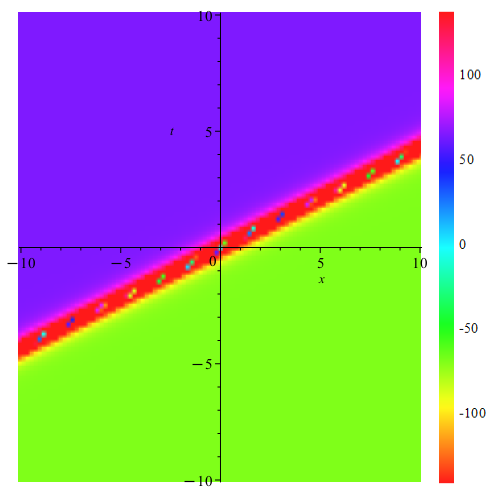
\includegraphics[width=\linewidth, height=55mm]{d4.png}\subcaption{} \end{minipage}
    \end{tabular}%
 \noindent\caption{The 3D, 2D and Density plots of $U_4(\xi)$ given by Eq. \ref{U4}.}\label{P4}
\end{figure}
\FloatBarrier
\section{Bifurcation Analysis}
In this section, the model under consideration is converted into a dynamical system via a Galilean transformation, enabling an examination of all potential phase portraits for the system. Using Eq. \ref{ODE1} we have
\begin{eqnarray}\label{ODE2}
U^{''}{(\zeta)}=\left(p^{2}+r \right) U \! \left(\zeta \right)-2 \gamma \! \left(U \! \left(\zeta \right)\right)^{3}.
\end{eqnarray}
We can write Eq. \ref{ODE2} as
\begin{eqnarray}\label{ODE3}
U^{''}{(\zeta)}=A\,U \! \left(\zeta \right)-B\,\! \left(U \! \left(\zeta \right)\right)^{3},
\end{eqnarray}
where $A={p^2+r}$ and $B={2\gamma}$.\\
It is established from references \cite{a34,a35} that Eq. \ref{ODE3} is analogous to the planar dynamical system\\
\begin{eqnarray}\label{BA}
\frac{d U}{d \zeta} = T,\nonumber
\end{eqnarray}
\begin{eqnarray}
\frac{d T}{d \zeta} = -B \,U^{3}+A U.
\end{eqnarray}
According to the theory of planar dynamical systems, the phase trajectories of Eq. \ref{BA} defines the precise traveling wave solutions for Eq. \ref{NLSE}. Consider a continuous solution $U(\zeta)$ of Eq. \ref{BA} satisfying ${\lim_{m\longrightarrow-\infty}U(\zeta)=P_{1}}$ and ${\lim_{m\longrightarrow\infty}U(\zeta)=P_{2}}$. Should $P_{1}$ equal $P_{2}$, then $U(\zeta)$ constitutes a homoclinic orbit, and consequently, $u(x, t)$ is a solitary wave solution. In the case where $P_{1} > P_{2}$,  forms a heteroclinic orbit, resulting in $u(x, t)$ being a kink wave solution; an antikink wave solution arises for  $P_{1} < P_{2}$. Furthermore, every closed curve within the phase portraits of Eq. \ref{BA}  corresponds to a periodic solution of Eq. \ref{NLSE}. To facilitate this analysis, the Hamiltonian function $H(U, T)$ is sought, defined such that $\frac{\partial H}{\partial T} = \mathit{U'}$  and $\frac{\partial T}{\partial \zeta} = -\mathit{T'}$ . This leads to the system
\begin{eqnarray}
\frac{\partial U}{\partial T} = T,\nonumber
\end{eqnarray}
\begin{eqnarray}
\frac{\partial H}{\partial U} =-T'= -(-B \,U^{3}+A U).
\end{eqnarray}
From Eq. \ref{BA}, it follows that $H(U, T)=\frac{T^2}{2}+f(U)$ where $f(U)$ is an arbitrary function of U. Consequently, $\frac{\partial H(U,T)}{\partial U} =-f'(U)$ and Integrating this yields $f(U)=B\,\frac{U^4}{4}-A\,\frac{U^2}{2}+a_{0}$ with $a_{0}$ as an arbitrary constant. Thus, the Hamiltonian is $H(U, T) = \frac{T^2}{2}+B\,\frac{U^4}{4}-A\,\frac{U^2}{2}+a_{0}$. By selecting the constant appropriately, one obtains\\
\begin{eqnarray}
H(U, V) = \frac{T^2}{2}+B\,\frac{U^4}{4}-A\,\frac{U^2}{2}=a_{1},
\end{eqnarray}
here, $T$ denotes the generalized momentum, $U$ the generalized coordinate, $\frac{T^2}{2}$ the kinetic energy, and $\,\frac{U^4}{4}-A\,\frac{U^2}{2}$ the potential energy, with $h_{1}$ representing the total energy constant.\\
The equilibrium points $E(U, T)$ for Eq. \ref{BA} are found by solving the system derived from setting $\frac{d U}{d \zeta}= 0$ and $\frac{d T}{d \zeta} = 0$
\begin{eqnarray}\label{EP}
0 = T,\nonumber
\end{eqnarray}
\begin{eqnarray}
0 = -B \,U^{3}+A U.
\end{eqnarray}
By using Eq. \ref{EP} obtain solutions for $U$. The first equation gives $T = 0$. The second equation yields $U=0$, $U=\sqrt{\frac{A}{B}}$ and $U=-\sqrt{\frac{A}{B}}$. Therefore, if $AB < 0$, the sole equilibrium point is $E_{1}(0, 0)$. If $AB > 0$, there exist three equilibrium points: $E_{1}(0, 0), E_{2}(\sqrt{\frac{A}{B}},0)$ and $E_{3}(-\sqrt{\frac{A}{B}}, 0)$.\\
The Jacobian matrix $J(U, T)$ for the Hamiltonian system at an equilibrium point $(U_{0},T_{0})$ is given by
\begin{eqnarray}
\frac{d U}{d \zeta} = \frac{\partial H}{\partial T},
\end{eqnarray}
\begin{eqnarray}
\frac{d T}{d \zeta} = -\frac{\partial H}{\partial U},
\end{eqnarray}
\begin{equation}
J(U, V) =
\begin{bmatrix}
\dfrac{\partial^2 H}{\partial U \, \partial T} & \dfrac{\partial^2 H}{\partial T^2} \\[8pt]
-\dfrac{\partial^2 H}{\partial U^2} & -\dfrac{\partial^2 H}{\partial T \, \partial U}
\end{bmatrix}_{(U_0, T_0)},
\end{equation}
For the specific system Eq. \ref{BA}, this evaluates to\\
\begin{center}
$J(U, V) =
\begin{bmatrix}
 0 & 1 \\[8pt]
 A-3\,B\,U^2 & 0
\end{bmatrix},$
\end{center}
with its determinant being
\begin{center}
$ |J (U, T)| = -(A-3\,B\,U^2).$
\end{center}
The bifurcations of phase portraits of system are displayed here\\
\begin{figure}[h!]
    \centering
    \begin{tabular}{ccc}
        \begin{minipage}{.30\textwidth} 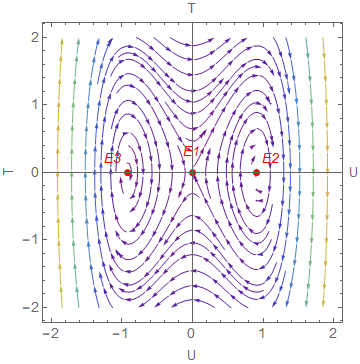
\includegraphics[width=\linewidth,
            height=55mm]{b1.png}\subcaption{} \end{minipage}
    \end{tabular}%
 \noindent\caption{The bifurcation of phase portrait of Eq. \ref{BA} for $A>0$ and $B>0$. }\label{B1}
\end{figure}\\
\begin{figure}[h!]
    \centering
    \begin{tabular}{ccc}
        \begin{minipage}{.30\textwidth} 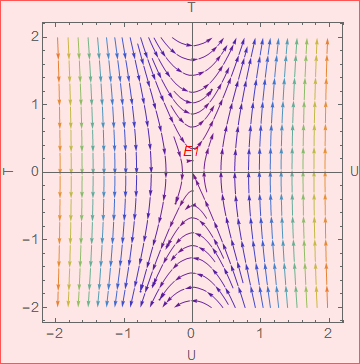
\includegraphics[width=\linewidth,
            height=55mm]{b2.png}\subcaption{} \end{minipage}
    \end{tabular}%
 \noindent\caption{The bifurcation of phase portrait of Eq. \ref{BA} for $A>0$ and $B<0$.}\label{B2}
\end{figure}\\
\begin{figure}[h!]
    \centering
    \begin{tabular}{ccc}
        \begin{minipage}{.30\textwidth} 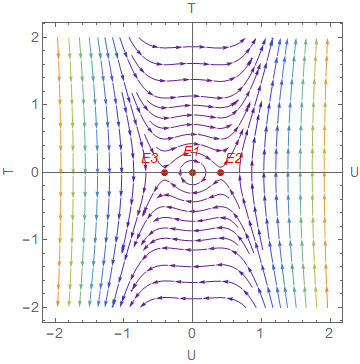
\includegraphics[width=\linewidth,
            height=55mm]{b3.png}\subcaption{} \end{minipage}
    \end{tabular}%
 \noindent\caption{The bifurcation of phase portrait of Eq. \ref{BA} for $A<0$ and $B>0$.}\label{B3}
\end{figure}\\
\begin{figure}[h!]
    \centering
    \begin{tabular}{ccc}
        \begin{minipage}{.30\textwidth} 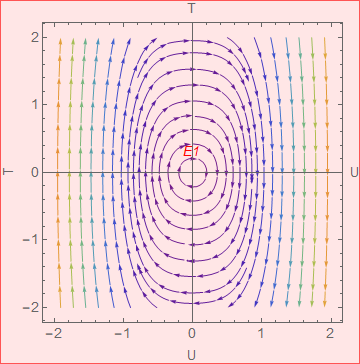
\includegraphics[width=\linewidth,
            height=55mm]{b4.png}\subcaption{} \end{minipage}
    \end{tabular}%
 \noindent\caption{The bifurcation of phase portrait of Eq. \ref{BA} for $A<0$ and $B<0$.}\label{B4}
\end{figure}
\noindent
\newpage
The bifurcation theory for planar dynamical systems provides the following classification, as stated in here\\
\textbf{Theorem:} For an equilibrium point $E(U_{0}, T_{0})$, if $|J(E)| < 0$, it is a saddle point, if $|J(E)| > 0$ and the $Trace(J(E)) = 0$, it is a center point and if $|J(E)| = 0$, $Trace(J(E)) = 0$, and its Poincare index is $0$, it is a cusp point.\\
Based on this, the bifurcation analysis for different parameter ranges is as follows:\\
\textbf{Preposition:}
\begin{itemize}
  \item \textbf{For $A > 0$, $B > 0$:} The system possesses three equilibrium points $E_{1}(0, 0), E_{2}(\sqrt{\frac{A}{B}},0)$ and $E_{3}(-\sqrt{\frac{A}{B}}, 0)$. The origin $E_{1}(0, 0)$ is a saddle point as $|J(E_{1})| < 0$ and a homoclinic orbit originates from and returns to the point $E_{1}(0, 0)$. The points $E_{2}(\sqrt{\frac{A}{B}},0)$ and $E_{3}(-\sqrt{\frac{A}{B}}, 0)$ are centers because $|J(E_{2,3})| > 0$ and $Trace(E_{2,3})=0$ each surrounded by a family of periodic orbits. The phase portrait of it is displayed in Fig. (\ref{B1}).
  \item \textbf{For $A > 0$, $B < 0$:} The only equilibrium point is $E_{1}(0, 0)$. This point is a saddle point $|J(E_{1})| < 0$. Consequently, no closed trajectories exist, meaning Eq. \ref{BA} has no periodic solutions. The phase portrait for different parameters is depicted in Fig. (\ref{B2}).
  \item \textbf{For $A < 0$, $B < 0$:} The system possesses three equilibrium points $E_{1}(0, 0), E_{2}(\sqrt{\frac{A}{B}},0)$ and $E_{3}(-\sqrt{\frac{A}{B}}, 0)$. The origin $E_{1}(0, 0)$ is a centre point as $|J(E_{1})| > 0$ and $Trace(E_{1})=0$ giving rise to a family of periodic orbits around it which correspond to periodic wave solutions for Eq. \ref{ODE3}. The points $E_{2}$ and $E_{3}$ are saddle points $|J(E_{2,3})| < 0$. The heteroclinic orbits connecting these saddles indicate the existence of solitary wave solutions. A representative phase portrait for arbitrary parameters is displayed in Fig. (\ref{B3}). A homoclinic orbit originates from and returns to the point $E_{1}(0, 0)$. The points $E_{2}(\sqrt{\frac{A}{B}},0)$ and $E_{3}(-\sqrt{\frac{A}{B}}, 0)$ are centers because $|J(E_{2,3})| > 0$ and $Trace(E_{2,3})=0$ each surrounded by a family of periodic orbits. The phase portrait of it is displayed in Fig. (\ref{B3}).
  \item \textbf{For $A < 0$, $B > 0$:} The only equilibrium point is $E_{1}(0, 0)$. This point is a center $|J(E_{1})| > 0$, $Trace=0$). All surrounding orbits are closed curves, indicating that Eq. \ref{ODE3} admits solely periodic solutions. The corresponding phase portrait with arbitrary parameters is presented in Fig. (\ref{B4}).
\end{itemize}
\section{Results and Discussion}\label{s4}
\noindent This paper will present new solutions to the non-linear Schr\"{o}dinger equation then those we have obtained using alternative methods. To the best of our knowledge, several solutions using  auxiliary equation method for the Schr\"{o}dinger problem are novel and have not been published in any literature. Proofs of analytic solutions for soliton waves, including hyperbolic functions, weakly acting functions, value functions, exponential functions and the triangular function solution problem of the Schr\"{o}dinger equation were found. The following observations can be used to explain the physical result of these solutions with 3D and 2D Contour density graphs by utilizing regular measurements and the suitable values of unknown coefficients. Fig. (\ref{P1}) shows the Dark soliton observed for Eq. \ref{U1}. Fig. (\ref{P2})  shows the Bright soliton  observed for Eq. \ref{U2}. Furthermore some similar solitory waves are also observed. Fig. (\ref{P3})  shows the Kink shaped soliton observed for Eq. \ref{U3}. The presentation of the analytical soliton solutions and dynamic behavior involves use of the appropriate values for the free parameter constants and unknown coefficients.\\
The traveling–wave reduction of the NLSE yields the second-order ODE
\begin{center}
    $U^{''}{(\zeta)}=A\,U \! \left(\zeta \right)-B\,\! \left(U \! \left(\zeta \right)\right)^{3},\quad A=p^2+r\quad, B=2\gamma$
\end{center}
which is recast as the planar Hamiltonian system
\begin{center}
    $U' = T, \qquad T' = -BU^3 + AU,$
\end{center}
with Hamiltonian $H(U,T) = \tfrac{1}{2}T^2 + \tfrac{B}{4}U^4 - \tfrac{A}{2}U^2.$ $H=$ constant generate the phase portraits and thus the traveling-wave solutions of the NLSE. The equilibria solve $T = 0, \; -BU^3 + AU = 0$, provides us $U^\ast \in \Big\{ 0, \; \pm \sqrt{\tfrac{A}{B}} \Big\}, \; \text{when } AB>0$,
and only $U^\ast = 0, \; \text{when } AB<0.$
Linearization via the Jacobian
    $J =
    \begin{bmatrix}
        0 & 1 \\
        A - 3B U^2 & 0
    \end{bmatrix}$
classifies the fixed points and determines the orbit topology.

%------------------------------
% Regimes
%------------------------------
\subsubsection*{Figure (\ref{B1}): $A>0, B>0$}
\begin{itemize}
    \item Three equilibria exist: the origin is a saddle $U^\ast = 0, \pm \sqrt{A/B}$
    \item The origin is a saddle: the non-zero equilibria are centers.
    \item Phase portrait: a separatrix homoclinic loop at the origin nested closed orbits around $\pm \sqrt{A/B}$.
    \item Solutions: solitary waves (homoclinic) and periodic traveling waves (around centers).
\end{itemize}

\subsubsection*{Figure (\ref{B2}): $A>0, B<0$}
\begin{itemize}
    \item Only $U^\ast = 0$, which is a saddle.
    \item No closed orbits: no periodic traveling waves.
    \item Solutions: separatrix-type connections.
\end{itemize}

\subsubsection*{Figure (\ref{B3}): $A<0, B<0$}
\begin{itemize}
    \item Equilibria: $U^\ast = 0, \pm \sqrt{A/B}$.
    \item The origin is a center: $\pm \sqrt{A/B}$ are saddles.
    \item Phase portrait: heteroclinic connections between the saddles and closed curves around the origin.
    \item Solutions: kink/antikink (fronts) and periodic waves.
\end{itemize}

\subsubsection*{Figure (\ref{B1}): $A<0, B>0$}
\begin{itemize}
    \item Only $U^\ast = 0$, which is a center.
    \item Phase portrait: closed orbits only.
    \item Solutions: periodic traveling waves only.
\end{itemize}
Bifurcation structure and physical meaning. Crossing the codimension-one sets $AB=0$ (creation/annihilation of the nonzero equilibria) and, separately, flipping the sign of
$A$ (curvature at the origin) reorganizes the phase portrait from “saddle-center-center” Fig. (\ref{B1}) to “single saddle” Fig. (\ref{B2}), to “center-saddle-saddle” Fig. (\ref{B3}) and to “single center” Fig. (\ref{B4}). Each reorganization switches the available waveform repertoire among \textbf{(i)} solitary pulses via homoclinic loops, \textbf{(ii)} periodic wavetrains via closed ovals and \textbf{(iii)} kinks/antikinks via heteroclinic connections. Mapping back to the NLSE parameters, $A=p^2+r$ couples carrier wave-number and frequency shift, while $B=2\gamma$ carries the nonlinearity sign; hence the observed transitions cleanly separate bright/dark-type solitary structures and periodic modulations according to the sign pattern of $(A,B)$. These portraits are consistent with the figures and propositions reported in the bifurcation section.
\section{Conclusion}\label{s5}
\noindent This work provides numerous new accurate soliton solutions and suggests using the auxiliary equation approach to solve the Schr\"{o}dinger problem. These new solutions may also help to clarify the physical properties of the given equation. Maple is used to verify the solutions that have obtained. This approach is found to be more broad, simple and intuitive which explains its efficacy, generative feature and suitability for handling a wide range of additional non-linear partial differential equations.\\
The bifurcation analysis of the traveling-wave dynamical system $U'' = AU - BU^3$ provides a complete classification of NLSE traveling solutions by the signs of $A = p^2+r$ and $B=2\gamma$. When both are positive, solitary pulses (homoclinic) and periodic wavetrains (centered ovals) co-exist when
\begin{itemize}
    \item $A>0, B>0$: solitary pulses (homoclinic) and periodic wavetrains coexist.
    \item $A>0, B<0$: only separatrix-type solutions, no periodic waves.
    \item $A<0, B<0$: kink/antikink fronts (heteroclinic) and periodic waves coexist.
    \item $A<0, B>0$: only periodic traveling waves exist.
\end{itemize}
Thus, sign changes in $(A,B)$ reorganize the phase space and determine the admissible coherent structures of the NLSE.
\begin{thebibliography}{99}
\bibitem{A1}Khater, A.H., Callebaut, D.K. and Abdelkawy, M.A. (2010). Two-dimensional force-free magnetic fields described by some nonlinear equations. \emph{Physics of Plasmas, 17}(12).
\bibitem{A2} Sodha, M.S., Konar,S. and Maheshwari, K.P. (1992). Steady-state self-focusing of rippled laser beams in plasmas: Arbitrary nonlinearity. \emph{Journal of plasma physics, 48}(1), 107-118.
\bibitem{A3} Bhrawy, A.H., Abdelkawy, M.A., Kumar, S., Johnson, S. and Biswas, A. (2013). Solitons and other solutions to quantum Zakharov–Kuznetsov equation in quantum magneto-plasmas. \emph{Indian Journal of Physics, 87}, 455-463.
\bibitem{a4}Srivastava, S. and Konar, S. (2009). Two-component coupled photovoltaic soliton pair in two-photon photorefractive materials under open circuit conditions. \emph{Optics and Laser Technology, 41}(4), 419-423.
\bibitem{a5}Konar, S., Kumar, J. and Sen, P.K. (1999). Suppression of soliton instability by higher order nonlinearity in long haul optical communication systems. \emph{Journal of Non-linear Optical Physics and Materials, 8}(04), 497-502.
\bibitem{a6}Konar, S. and Jana, S. (2004). Linear and non-linear propagation of sinh-Gaussian pulses in dispersive media possessing Kerr nonlinearity. \emph{Optics communications, 236}(1-3), 7-20.
\bibitem{a7}Jana, S. and Konar, S. (2007). A new family of Thirring type optical spatial solitons via electromagnetically induced transparency. \emph{Physics Letters A, 362}(5-6), 435-438.
\bibitem{a8}Bhrawy, A. and Abdelkawy, M. (2013). Computational study of some nonlinear shallow water equations. Open Physics, 11(4), 518-525.
\bibitem{a9}Bhrawy, A.H., Tharwat, M.M. and Abdelkawy, M.A. (2013). Integrable system modelling shallow water waves: Kaup–Boussinesq shallow water system. \emph{Indian Journal of Physics, 87}, 665-671.
\bibitem{a10}Ghosh, S. and Nandy, S. (1999). Inverse scattering method and vector higher order non-linear Schrödinger equation. \emph{Nuclear Physics B, 561}(3), 451-466.
\bibitem{a11}Bhrawy, A.H., Biswas, A., Javidi, M., Ma, W.X., Pinar, Z. and Yildirim, A. (2013). New solutions for (1+ 1)-dimensional and (2+ 1)-dimensional Kaup–Kupershmidt equations. \emph{Results in Mathematics, 63}, 675-686.
\bibitem{a12}Sakthivel, R., Chun, C. and Bae, A.R. (2010). A general approach to hyperbolic partial differential equations by homotopy perturbation method. \emph{International Journal of Computer Mathematics, 87}(11), 2601-2606.
\bibitem{a13}Wazwaz, A.M. (2008). The Hirota’s bilinear method and the tanh–coth method for multiple-soliton solutions of the Sawada-Kotera-Kadomtsev-Petviashvili equation. \emph{Applied Mathematics and Computation, 200}(1), 160-166..
\bibitem{a14}Wang, M., Zhou, Y. and Li, Z. (1996). Application of a homogeneous balance method to exact solutions of non-linear equations in mathematical physics. \emph{Physics Letters A, 216}(1-5), 67-75.
\bibitem{a15}Khater, A.H., Callebaut, D.K., Bhrawy, A.H. and Abdelkawy, M.A. (2013). Non-linear periodic solutions for isothermal magnetostatic atmospheres. \emph{Journal of Computational and Applied Mathematics, 242}, 28-40.
\bibitem{a16}Liu, S., Fu, Z., Liu, S. and Zhao, Q. (2001). Jacobi elliptic function expansion method and periodic wave solutions of non-linear wave equations. \emph{Physics Letters A, 289}(1-2), 69-74.
\bibitem{a17}Zhou, Y., Wang, M. and Miao, T. (2004). The periodic wave solutions and solitary wave solutions for a class of non-linear partial differential equations. \emph{Physics Letters A, 323}(1-2), 77-88.
\bibitem{a18}Wazwaz, A.M. (2008). A study on linear and non-linear Schr\"{o}dinger equations by the variational iteration method.\emph{ Chaos, Solitons and Fractals, 37}(4), 1136-1142.
\bibitem{a19}Zhang, H.Q., Tian, B., Li, L.L. and Xue, Y.S. (2009). Darboux transformation and soliton solutions for the (2+ 1)-dimensional non-linear Schrödinger hierarchy with symbolic computation. \emph{Physica A: Statistical Mechanics and its Applications, 388}(1), 9-20.
\bibitem{a20}Pawlik, M. and Rowlands, G. (1975). The propagation of solitary waves in piezoelectric semiconductors. \emph{Journal of Physics C: Solid State Physics, 8}(8), 1189.
\bibitem{a21}Pedlosky, J. (1970). Finite-amplitude baroclinic waves. \emph{Journal of the Atmospheric Sciences, 27}(1), 15-30.
\bibitem{a22}Wadati, M., Segur, H. and MJ, A. (1992). A new Hamiltonian amplitude equation governing modulated wave instabilities. \emph{Journal of the Physical Society of Japan, 61}(4), 1187-1193.
\bibitem{a23}Beuß, H. (1996). On unstable non-linear Schrödinger equations. \emph{Non-linear Analysis: Theory, Methods and Applications, 26}(5), 903-914.
\bibitem{a24}Arnold, A. (1998). Numerically absorbing boundary conditions for quantum evolution equations. \emph{VLSI design, 6}(1-4), 313-319.
\bibitem{a25}Dehghan, M. and Shokri, A. (2007). A numerical method for two-dimensional Schrödinger equation using collocation and radial basis functions. \emph{Computers and Mathematics with Applications, 54}(1), 136-146.
\bibitem{a26}Tappert, F.D. (2005). The parabolic approximation method. \emph{Wave propagation and underwater acoustics}, 224-287.
\bibitem{a27}Huang, W., Xu, C., Chu, S.T. and Chaudhuri, S.K. (1992). The finite-difference vector beam propagation method: analysis and assessment. \emph{Journal of Lightwave Technology, 10}(3), 295-305.
\bibitem{a28}Hajj, F.Y. (1985). Solution of the Schr\"{o}dinger equation in two and three dimensions. \emph{Journal of Physics B: Atomic and Molecular Physics, 18}(1), 1.
\bibitem{a29}Gagnon, L., Grammaticos, B., Ramani, A. and Winternitz, P. (1989). Lie symmetries of a generalised non-linear Schr\"{o}dinger equation. III. Reductions to third-order ordinary differential equations. \emph{Journal of Physics A: Mathematical and General, 22}(5), 499.
\bibitem{a30}Gagnon, L. and Paré, C. (1991). Non-linear radiation modes connected to parabolic graded-index profiles by the lens transformation. \emph{JOSA A, 8}(4), 601-607.
\bibitem{a31}Gagnon, L. and Winternitz, P. (1989). Lie symmetries of a generalised non-linear Schr\"{o}dinger equation. II. Exact solutions. \emph{Journal of Physics A: Mathematical and General, 22}(5), 469..
\bibitem{a32}Gagnon, L. and Winternitz, P. (1989). Exact solutions of the spherical quintic non-linear Schrödinger equation. \emph{Physics Letters A, 134}(5), 276-281.
\bibitem{a33}Gagnon, L. and Winternitz, P. (1990). Non-Painlevé reductions of non-linear Schrödinger equations. \emph{Physical Review A, 42}(8), 5029.
\bibitem{a34}Li, J. and Liu, Z. (2002). Traveling wave solutions for a class of nonlinear dispersive equations. \emph{Chinese Annals of Mathematics, Series B, 23}(3), 397–418.
\bibitem{a35} Liang, J., Tang, L., Xia, Y. and Zhang, Y. (2020). Bifurcations and exact solutions for a class of MKdV equations with the conformable fractional derivative via dynamical system method. \emph{International Journal of Bifurcation and Chaos, 30}(1), 2050004.
\end{thebibliography}
\end{document}  